\documentclass[t]{beamer}
\input{\jobname_header}
\input{\jobname_beameranpassungen}

\NewDocumentCommand{\altTeX}{}{%
  \textsf{alt}\TeX\xspace
}


\begin{document}

\section{Maschinen}
\begin{frame}{Was haben \TeX\ und Tastaturbelegungen gemeinsam?}
•<+> Sie sind alt!
• die am weitesten verbreitete Belegung |qwerty/z| kam 1868 auf
• \TeX\ kam 1978 in der ersten Version raus
• seitdem hat sich bei \TeX\ einiges getan – bei Tastaturen nicht
• da die Tastatur das wichtigste Hilfsmittel ist – betrachten wir die Entwicklung der beiden Ts und schauen, wie sie voneinander profitieren können
\•
\end{frame}

% ⇒ overview

\begin{frame}{Vorteile neuer Maschinen}
• lua\TeX\ und \XeTeX\ unterstützen nativ und vollständig utf8
•[⇒] nie mehr Probleme beim Austausch von Dokumenten, nie wieder kaputte Umlaute, keine umständliche Eingabe von speziellen Zeichen anderer Sprachen
• ganz zu schweigen von asiatischem Satz …
• lua\TeX\ und \XeTeX\ unterstützen nativ moderne Schrifttechnologien ⇒ es werden keine speziellen Dateien zum Schrifteinbinden benötigt
•[⇒] modernste, neuste Schriften sind in vollem Funktionsumfang verfügbar
• Wermutstropfen bei \XeTeX: Mikrotypographie nicht wie bei pdf\TeX\ möglich, daher oft vernachlässigt in der Wahl der Maschine
• aber Vorteil: unterstützt |pstricks|!
\•
\end{frame}

\section{Formate}
\begin{frame}{Formate}
• fast niemand verwendet INITEX als Programm
• fast immer wird ein Format verwendet:
• plain\TeX: Do It Yourself!
• \LaTeX: A Document Preparation Program
• Con\TeX t: The super-duper cow power
\•
\end{frame}

\begin{frame}{The neverending story: \LaTeX3}   %% hat 448 Seiten und auch ein Ende …
• \LaTeXe: eigentlich als Zwischenversion zu \LaTeX3 geplant, inzwischen eingefroren und meistverwendetes \TeX-Format
• keine Weiterentwicklung im Kernel, keine Korrektur von Designfehlern
• \LaTeX3 als lange währendes, unbekanntes Mysterium …
• einige Pakete bauen bereits auf \LaTeX3-Code auf
• z.\,B. |siunitx|, |fontspec|
• inzwischen ist \LaTeX3 sogar bei lua\TeX\ angekommen …
\•
\end{frame}

\begin{frame}{Con\TeX t}
• baut in der neusten Verison voll auf lua\TeX\ auf
• kann alles außer Dokumentation
• wer mag, darf nun was dazu sagen …
\•
\end{frame}

\begin{frame}{Designmerkmale von \LaTeX3 (Auswahl)}
• Versuch einer „gesunden“ (sane) Programmierebene, die von \TeX\ abstrahiert
• gute, übersichtliche Namensgebung von internen Makros (großes Problem von \LaTeXe)
• sinnvolle Strukturierung etc. etc. etc.
\•
\end{frame}

\begin{frame}[fragile]{Designmerkmale von \LaTeX3 (Auswahl)}
• Namen: Das |@| als Trennstelle in Namen wird vom |_| übernommen
• Interne Namen enden mit einem |:|
• Nach dem |:| werden erwartete Argumente benannt: |\cs_new:Npn|
\• 
\end{frame}

\begin{frame}[fragile]{Beispiel für sinnvolle \LaTeX3-Konstrukte}
• angenommen: Der Nutzer kann einen Namen |\name| vorgeben. Aus diesem Namen werden die Befehle |name1|, |name2| und |name-<name1>| gebaut. (|hallo| ⇒ |hallo1|, |hallo2|, |hallo-Inhalt 1|)
\•
\begin{block}{\TeX, meist in \LaTeX\ verwendet:}
\begin{verbatim}
\expandafter\def\csname \name1\endcsname{Inhalt 1}
\expandafter\def\csname \name2\endcsname{Inhalt 2}
\expandafter\def\csname \name-\csname\name \endcsname\endcsname{Inhalt von name-<name>}
\end{verbatim}
\end{block}

\begin{block}{\LaTeX3}
\begin{verbatim}
\ExplSyntaxOn
\cs_new:cpn{\name1}{Inhalt 1}
\cs_new:cpn{\name1}{Inhalt 2}
\cs_new:cpn{\name1-\cs:w \name \cs_end:}{Inhalt 1}
\ExplSyntaxOff
\end{verbatim}
\end{block}
\end{frame}

\begin{frame}{\LaTeXe-Versionen}
\LaTeXe\ bietet z.\,B. |\@nameuse| und |\@namedef|, aber das nutzt niemand … weil es niemand kennt und es nicht konsequent ist.\\
(Kannte ich bis eben auch nicht …)
\end{frame}

\begin{frame}[fragile]{Beispiel für Paketschreiben mit \LaTeX3}{levelscheme.dtx}
• bestes Beispiel für Arbeit mit \LaTeX3: \LaTeX3 …
• für alles andere: |expl3| unter \LaTeXe
• |expl3| bietet grundlegendes Programmierinterface
• bietet viele Lösungen, für die \LaTeXe\ nur sehr umständliche Konstrukte hatte
\•
\begin{verbatim}   %%% oder so ähnlich und so …
\expandafter\let\expandafter\second\first
\cs_set_eq:Ne\second\first
\end{verbatim}
\end{frame}

\section{Neo – ein Tastaturlayout}
\begin{frame}{Tastaturbelegungen – ganz kurz}
• Anordnung der Tasten, Zeichenauswahl etc. noch von uralten Schreibmaschinen beibehalten
• nur wenige, kleine Änderungen (|y| und |z| im Deutschen getauscht, Umlaute)
• kaum Rücksichtnahme auf Erogonomie
• Belegung durch mechanische Bedingungen gegeben
\•
\end{frame}

\begin{frame}[fragile]{Neo – ein Tastaturlayout}
• Hauptziel: ergonomische Tastaturbelegung
• schnelles Schreiben (auch mit unergonomischen Belegungen möglich)
• angenehmes Schreiben (geringe Laufwege für Finger entlasten Gelenke)\pause
• Nebenziel/Nebeneffekt: Große Vielzahl an Sonderzeichen leicht erreichbar
• Ergonomie: statt Rumklicken oder Zahleneingabe: Tastenkombination\\%
|Ξ√Λℂ⊂∫∀∃∪∩ΠℵΨΓΦℚ⇔↦⇒ΣΔ … |
\•
\end{frame}

\begin{frame}[fragile]{Neo – ein Tastaturlayout mit vielen Sonderzeichen}
• erreichbar über zusätzliche Modifier
• maximal zwei Modifier plus Taste
• für noch mehr Sonderzeichen: Compose-Taste\\%
(unter Linux und Solaris bekannt, jetzt auch für Windows, und stark erweitert)
\•
\end{frame}

\begin{frame}{Neo – Ebenen 1 und 2:}
\input{ebene12}
\end{frame}

\begin{frame}{Neo – Ebene 3:}
\input{ebene3}
\end{frame} 

\begin{frame}{Neo – Ebene 6:}
\input{ebene6}
\end{frame} 

\section{Experimente mit \altTeX}
\begin{frame}{Was ist \altTeX?}
• experimentelles Paket zum „alternativen \TeX en“
• Ansätze, die häufige Arbeiten einfacher machen
• stark auf Neo aufbauend (Verwendung vieler unicode-Zeichen)
• 
\•
\end{frame}

\begin{frame}[fragile]{Itemize}
• Aufzählung im normalen Text:
\begin{verbatim}
\begin{itemize}
\item erster Punkt
\item zweiter Punkt
\end{itemize}
\end{verbatim}
• recht viel Schreibarbeit
• ein guter Editor kann sehr viel Arbeit abnehmen
• aber Code schlecht lesbar
\•
\end{frame}

\begin{frame}[fragile]
• Idee: Nehme ein freies Unicodezeichen (z.\,B. |•|)
• weise dem Zeichen eine Bedeutung zu, die seinem Aussehen entspricht (z.\,B. Aufzählungspunkt)
• implementiere so, dass kein weiterer Code nötig ist (Umgebungen etc.)
\•
\end{frame}

\begin{frame}[fragile]{Beispiel: itemize}
• Ziel: der Code soll genau das tun, wonach er aussieht:
\begin{verbatim}
normaler Text

• erster Punkt
• zweiter Punkt

weiter im Text
\end{verbatim}
•[⇒] Äufzahlung ohne weitere \TeX-Befehle
\•
\end{frame}

\begin{frame}[fragile]{Beispiel: itemize}
• erster Ansatz: |•| aktiv machen
\begin{verbatim}
\catcode\`• = \active
\end{verbatim}
\pause
• Bedeutung zuweisen:
\begin{verbatim}
\let • \item
\end{verbatim}
• Bereits Verbesserung im Lesefluss:
\begin{verbatim}
\begin{itemize}
• erster Punkt
• zweiter Punkt
\end{itemize}
\end{verbatim}
\•
\end{frame}

\begin{frame}[fragile]{Beispiel: itemize}
• weiterhin: Umgebung |\begin{verbatim}| einsparen!
• dazu: bei jedem Auftreten von |•| prüfen, ob man bereits in der Aufzählung ist:\pause
\•
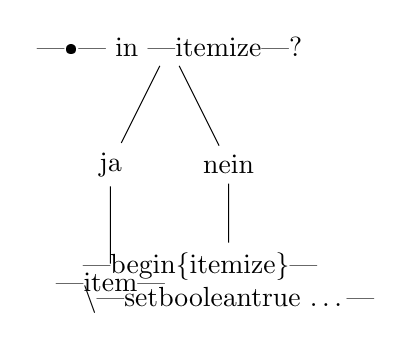
\begin{tikzpicture}
\node {|•| in |itemize|?}
    child {node {ja}
      child {node {|item|}}}
    child {node {nein}
      child {node {\vbox{\hbox{|begin\{itemize\}|}\hbox{\textbackslash|setbooleantrue …|}}}}}
;
\end{tikzpicture}
\end{frame}

\begin{frame}[fragile]{Beispiel: itemize}
• schließlich: |\end{verbatim}| einsparen
• Problem: kein Zeichen zum Beenden verwendet!
•[⇒] wann weiß \TeX, dass die Umgebung beendet werden soll?\pause
• Ansatz: Eindeutige Sequenz beendet die Umgebung: Doppeltes Zeilenende (= Leerzeile)
•[⇒] definiere Zeilenende als Makro, das überprüft, ob es ein- oder zweimal aufgetreten ist
• falls zweimal: beende Umgebung und setze Zeilenende auf normale Bedeutung zurück
\•
\end{frame}

\begin{frame}[fragile]
\begin{verbatim}
\cs_new:Npn\newitemi{%
  \if_meaning:w\insideitemizei\inside%
    \cs_set_eq:NN\altlastitem1%
    \exp_after:wN\item%
  \else:%
    \begin{itemize}%
    \cs_set_eq:NN\insideitemizei\inside%
    \cs_set_eq:NN\altlastitem1%
    \makeenteractive%
    \exp_after:wN\item%
  \fi:
}
\end{verbatim}
\end{frame}

\begin{frame}[fragile]{\altTeX für den Mathesatz}{Unicodezeichen im Mathesatz}
• Schreiben von Unicodezeichen als Mathesatz: Paket |unicode-math| von Will Robertson\pause
• Ermöglicht direkte Eingabe aller mathematischen Zeichen unter Verwendung von OpenType-Matheschriften
• |∫₀⁸ x² = 170 ⅔|
\•
\end{frame}

\begin{frame}[fragile]{\altTeX für den Mathesatz}{Hoch- und Tiefstellen}
• Schreiben vieler hoch- und tiefgestellter Zahlen (z.\,B. Tensorrechnung) ist sehr lästig
•[⇒] Ziel: Einsparen von Gruppierungen!
• Ansatz: Definiere |_| und |^| als Makros, die ihr Argument bis zum nächsten Leerzeichen suchen, falls keine Klammer geöffnet wird
• Alles zwischen |_|,|^| und einem Leerzeichen wird als Argument hoch- bzw. tiefgestellt
• erspart immens viel lästige Schreibarbeit
• nur für kurze Argumente geeignet, da aber am nützlichsten
• bei langen Argumenten: wie üblich gruppieren
\•
\end{frame}

\begin{frame}[fragile]{\altTeX für den Mathesatz}{Klammersetzen}
• Klammern müssen fast immer mit |\left| und |\right| gesetzt werden:
\•
\begin{LTXexample}
\[(\frac 12) \left(\frac 12 \right)\]
\end{LTXexample}
•[⇒] Ziel: Klammern werden immer angepasst
• Ansatz: Sichere Bedeutung von |()| in Makros |\openbrace \closebrace|
• mache |()| aktiv
• definiere |()| als |\left\openbrace| bzw. |\right\openbrace|\pause
• Problem: Jegliche andere Verwendung von Klammern (im Text, bei |picture|-Umgebung u.\,ä.) funktioniert nicht mehr!
• Abfangen durch geschicktere Definition, Überprüfen des Mathemodus etc.
\•
\end{frame}

\begin{frame}[fragile]{\altTeX für den Mathesatz}{Matrizen}
• Eingabe von Matrizen ist recht aufwändig und unübersichtlich:
\•
\begin{LTXexample}
$\begin{bmatrix} a & b \\ c & d \end{bmatrix}$
\end{LTXexample}
• Unicode verfügbt über Klammern, die zum Einschließen von Matrizen geeignet sind
• mit Neo leicht zu erzeugen über Compose-Funktion:
\•
\begin{verbatim}
♫ x <Klammertyp> <Anzahl Spalten>
♫ x ( 3
⎛⎞
⎜⎟
⎝⎠
\end{verbatim}
\end{frame}


\begin{frame}[fragile]{\altTeX für den Mathesatz}{Matrizen}
• Idee: wieder aktive Zeichen
• erstes Klammerzeichen (links oben) beginnt die Matrix, setzt andere Zeichen auf die entsprechenden Makros
• alle rechten Klammerzeichen sorgen für einen Zeilenumbruch in der Matrix
• zur Sicherheit: rechte Klammerzeichen ignorieren das nächste Zeichen ⇒ verhindert Doppelausführung, falls rechte und linke Begrenzungen identische Zeichen sind
• das letzte rechte Zeichen beendet die Matrix
\•
\end{frame}

\begin{frame}[fragile]{\altTeX für den Mathesatz}{Matrizen}
• weitere mögliche Verbesserung: Definiere den Tabulator als Zellentrennzeichen |&| ⇒ keine Steuerzeichen stören die Matrix, sie passt hervorragend ins Dokument, an Tabulatoren ausgerichtet\pause
• Nachteil: Schreiben mitten in der Zeile ist nicht möglich, da \TeX\ zeilenweise einliest:
\•
\begin{verbatim}
a  = ⎛⎞
     ⎜⎟
     ⎝⎠ + b
\end{verbatim}
Außerdem keine Matrizen mit verschiedenen Klammern möglich ⇒ ließe sich aber implementieren, wenn die Eingabe möglich wäre.
\end{frame}

\end{document}












